\section{Evaluation}
\subsection{Data Sets}
We experiment our model on two datasets. The first one is proposed by \cite{luo2016temporal} and aims at extraction relations between entity and time (\emph{time RE data}). The dataset is constructed by aligning Wikidata triples with Wikipedia corpus. Based on the granularity of the time expression in the sentence, this dataset can be split into 3 subsets with different levels of reliability. The reliable subset is used as basic training data, validation data and test data which contains 22,214, 2,776 and 2,771 positive sentences respectively. The two less reliable subset contains 2,094 and 53,469 positive sentences and are used as additional training data. Negative data are constructed with two heuristic strategies. We use this dataset because this is a public dataset on relation extraction that has both reliable and unreliable data, which is suitable for all of our experiment settings.

We also conduct our experiment on the dataset proposed by \cite{riedel2010modeling}, which is a commonly used dataset in relation extraction (\emph{entity RE}). This dataset is generated by aligning triples in Freebase with the New York Times corpus (NYT corpus). The training data contains 522,611 sentences and 281,270 entity pairs. The test set contains 172,448 sentences and 96,678 entity pairs. We experiment our bag level models in this dataset to see the generalization ability of our transition matrix model.


\subsection{Hyper-parameters}
\paragraph{Sentence Level Model}
We experiment our sentence level model on time RE data. We use 100-dimensional word embedding pre-trained using GloVe \cite{pennington2014glove} on Wikipedia and Gigaword, and 20-dimensional vector for distance embedding. The convolution window is 3 and the number of convolution kernels is 200. The size of the full connection layer is also 200. As for training, we use stochastic gradient descend (SGD) for optimization with batch size 20, learning rate 0.1. We also use dropout with probability 0.5 upon the sentence embedding. Each phase of the curriculum learning over dataset contains 15 epochs. The trace normalization parameters for three subsets are $\beta_1=-0.01$, $\beta_2=0.01$ and $\beta_3=0.1$ (the ratio of $\beta_3$ and $\beta_2$ is fixed to 10 and 5 when tuning hyper-parameters).

\paragraph{Bag Level Model}
The parameters of the bag level model is almost the same as the sentence level model on time RE data, except that the learning rate is 0.01. As for entity RE data, our settings for prediction branch is similar to \cite{lin2016neural}. The word embedding is of dimension 50 and is pre-trained on the NYT corpus using word2vec\footnote{\url{ https://code.google.com/p/word2vec/}}. The convolution window is 3 and the number of convolution kernels is 256, distance embedding size is 5, batch size is 16 and learning rate is 0.01. For all the bag level models, the linear combination parameter $\alpha$ is 1 and trace normalization parameter $\beta$ is -0.1 at the start of training. We experiment with decay rate \{0.95, 0.9, 0.8\} and decay step \{3, 5, 8\}. We find that using decay rate 0.9 and decay step 5 performs well in most situations.

\begin{figure}[htbp]
\begin{center}
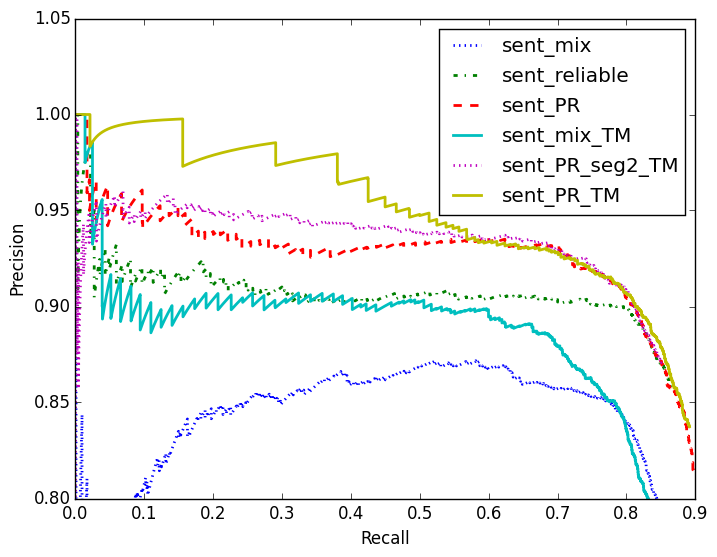
\includegraphics[width=0.9\linewidth]{figures/sent_time_exp_overall.png}
\caption{Sentence Level Results on Time RE}
\label{fig: sent_luo}
\end{center}
\end{figure}

\subsection{Results on Time RE Data}
We exhibit the results in the form of precision recall curves (PR curves).

\paragraph{Sentence Level Models}
The results of sentence level models is shown in Figure \ref{fig: sent_luo}. We can see that the performance of the model trained on all subsets mixed together (\emph{sent\_mix}) is very bad, which is significantly worse than the model trained only on the reliable subset (\emph{sent\_reliable}). This shows that the noise problem is innegligible and have bad influence on the training of the model. However, with the help of transition matrix, the model obtains the ability of modeling noise (\emph{sent\_mix\_TM}), which significantly improves the performance of the model. By using the reliable subset first and gradually adding less reliable data (\emph{sent\_curr}), we can see that the model can actually make use of the noisy data and performs better than the model trained only on the reliable subset. If we further use the transition matrix under the curriculum learning framework (\emph{sent\_curr\_TM}), the transition matrix will model the noise better and further improve the model performance. Apart from the experiments above, we also experiment our model in the situation where all the unreliable data are merged into one subset (\emph{sent\_seg2\_curr\_TM}), which means there are only two subsets: reliable subset and unreliable subset. We conduct this experiment because this setting will reduce the hyper-parameters and make the training easier to perform. We can see the, although this setting is not as good as using the full information of the data quality (using 3 subsets), it still has reasonable performance and also significantly outperforms the model which only use curriculum learning over dataset.


\begin{figure*}[htbp]
\centering
\subfigure[Attention Aggregation]{
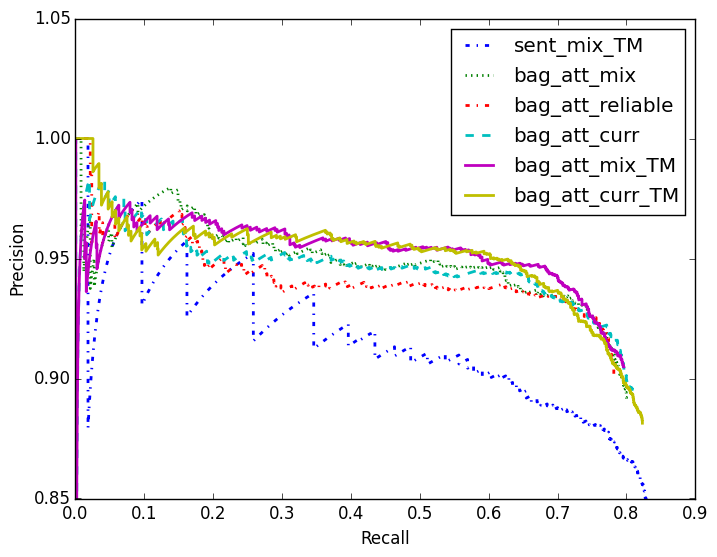
\includegraphics[width=0.45\linewidth]{figures/bag_att_exp_overall.png}
\label{fig: bag_att_luo}
}
\subfigure[Average Aggregation]{
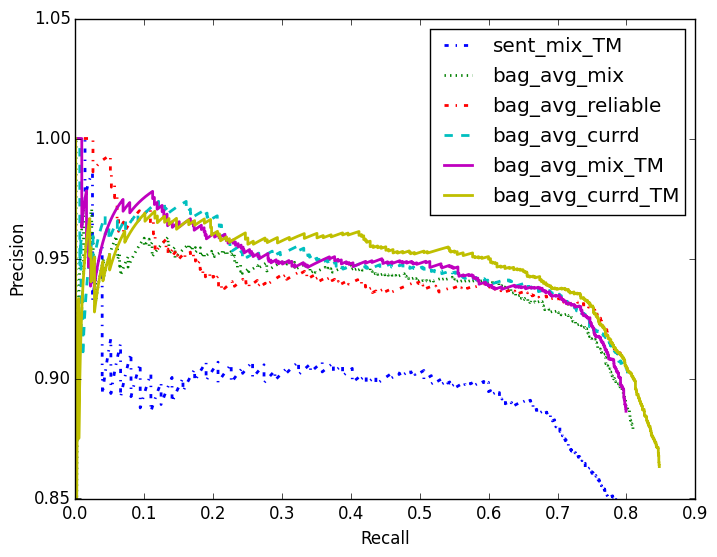
\includegraphics[width=0.45\linewidth]{figures/bag_avg_exp_overall.png}
\label{fig: bag_avg_luo}
}
\caption{Bag Level Results on Time RE}
\label{fig: results_on_luo}
\end{figure*}

\paragraph{Bag Level Attention Aggregation Models}
The results of the bag level models with attention aggregation is shown in Figure \ref{fig: bag_att_luo}. We can see that the basic bag level attention aggregation model (\emph{bag\_att\_mix}) performs very good and significantly outperforms the \emph{sent\_mix\_TM} model. Recall that the bag level model is based on the at-least-one assumption that at least one of the sentences in the sentence bag support the ($subj$, $rel$, $obj$) triple, and the \emph{sent\_mix\_TM} model do not use any assumption about the dataset. This shows that prior knowledge of the data quality plays an important role in the situation where the dataset is noisy. In the bag level models, the curriculum learning over dataset can be conducted by using only the reliable sentences in the sentence bag, and add unreliable sentences gradually. However, we find that using only reliable subset (\emph{bag\_att\_reliable}) or using curriculum learning over dataset alone (\emph{bag\_att\_curr}) does not improve the bag level attention aggregation model. This shows that the less reliable data in the sentence bag may provide additional side information or possibly plays the role of avoiding overfitting. \todo{polish the explanation.} Also note that the at-least-one assumption does not always hold and there are also false negative and false positive problems in bag level. Therefore, we can see that using transition matrix with or without curriculum learning over the dataset (\emph{bag\_att\_curr\_TM} and \emph{bag\_att\_mix\_TM}) all improve the model performance, and the \emph{bag\_att\_curr\_TM} model performs better in the low recall region.

\paragraph{Bag Level Average Aggregation Models}
The results of the bag level models with average aggregation is shown in Figure \ref{fig: bag_avg_luo}. The ranking of each setting is similar to the attention aggregation models. One interesting thing is that our transition matrix method improves the average aggregation models more significantly than the attention aggregation models. Note that the average aggregation model actually do not have good ability of handling sentence level noise. Therefore, the unhandled sentence level noise may further propagate to the bag level, which gives the transition matrix more chance to help model the noise. Also note that the \emph{bag\_avg\_curr\_TM} model significantly outperforms the \emph{bag\_avg\_mix\_TM}, this shows that curriculum learning over dataset helps the transition matrix more when the noise is more severe.

\begin{figure}[htbp]
\begin{center}
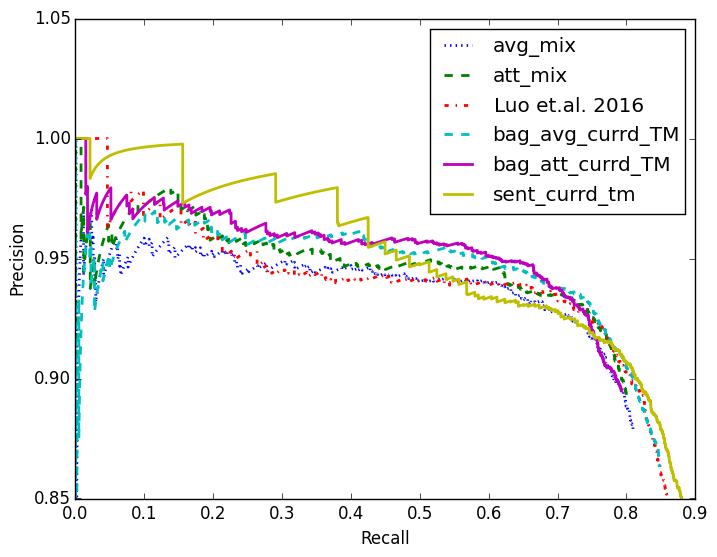
\includegraphics[width=0.9\linewidth]{figures/best_cmp_exp_overall.png}
\caption{Comparison on Time RE}
\label{fig: cmp_luo}
\end{center}
\end{figure}

\paragraph{Comparison}
\todo{polish this part}
The comparison of the best settings of each model family is shown in Figure \ref{fig: cmp_luo}. We can see that all of our models outperforms the model of \cite{luo2016temporal}. With the help of transition matrix, although the basic version of average aggregation is not as good as attention aggregation, its transition matrix version is similar to the attention aggregation. Also note that although the sentence level models trained on mixed data do not perform very good, the sentence level model can use transition matrix to model the sentence level noise and thus performs best in all these models. Recall that the transition matrix can model the noise rather than just reduce the influence of noisy sentences as in bag level models, the sentence level model actually has the ability to make use of the noisy data. This shows that sentence level noise is more important than the bag level noise in relation extraction, and modeling noise works better than just trying to reducing the influence of noise.


\begin{figure}[htbp]
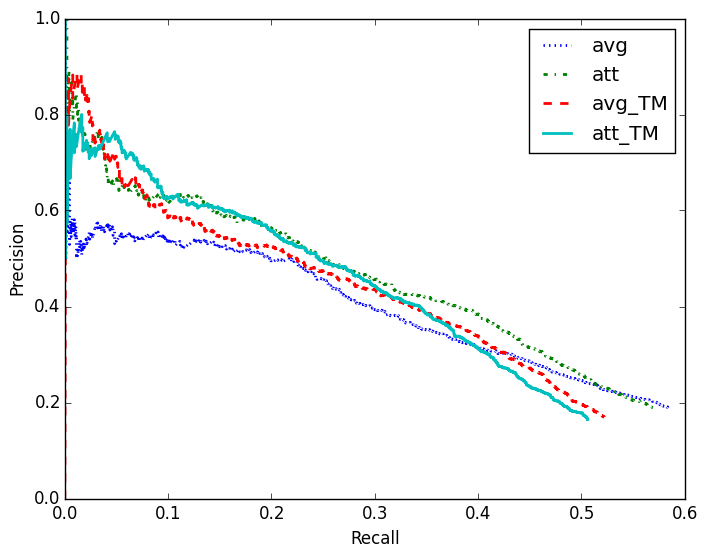
\includegraphics[width=0.9\linewidth]{figures/re_att_avg_cmp_exp.png}
\caption{Results on Dataset of Riedel et.al.}
\label{fig: Riedel_res}
\end{figure}

\subsection{Performance on Entity RE Data}
To show the generalization ability of our proposed transition matrix method, we also conduct experiments on the entity RE dataset proposed by \cite{riedel2010modeling}, which is a commonly used dataset in relation extraction. We implement the average aggregation method (\emph{avg}) and the attention aggregation method (\emph{att}) proposed by \cite{lin2016neural} as well as the corresponding transition matrix version (\emph{avg\_TM} and \emph{att\_TM}). The results are shown in Figure \ref{fig: Riedel_res}. We can see that, since the average aggregation method do not have good ability in handling sentence level noise, it performs significantly worse than the attention aggregation method. Similar to the results in time RE data, since the unhandled sentence level noise propagates to the bag level, which makes the bag level noise become more severe, the transition matrix has more chance to model the noise. Therefore, the \emph{avg\_TM} model significantly outperforms the \emph{avg} model. As for attention aggregation, this model already have good ability in reducing the impact of sentence level noise. Since the bag level noise is less important than the sentence level noise, the improvement of our transition matrix model is limited, which only improves the model on the low recall part. Note that the low recall part corresponds to high precision, which is more useful than the rest of the extraction results in practice. Therefore, our transition matrix method is also useful in this situation.

\iffalse
\begin{figure*}[htbp]
\centering
\subfigure[Overall PR Curves]{
\includegraphics[width=0.475\linewidth]{figures/reg_exp_overall.png}
\label{fig: reg_overall_pr_curve}
}
\subfigure[Small Relation PR Curves]{
\includegraphics[width=0.475\linewidth]{figures/reg_exp_small.png}
\label{fig: reg_small_rel_pr_curve}
}
\caption{Impact of Regularization Weights}
\label{fig: reg_PR_curve}
\end{figure*}
\fi